\documentclass[a4paper]{article}
\usepackage[utf8]{inputenc}
\usepackage[english]{babel}
\usepackage[T1]{fontenc}
\usepackage{graphicx}
\usepackage{lmodern}

\usepackage[
	left=2cm,
	right=2cm,
	top=1.2cm,
	bottom=2cm,
	% showframe % Muestra un marco alrededor del texto
	]{geometry}

\usepackage{microtype}
%\usepackage{lipsum}
%\usepackage{blindtext} % Como lipsum, pero con más funciones
\usepackage{float}
\usepackage{emptypage}
%\usepackage{sectsty} % Permite cambiar el aspecto del título de las secciones.
%\allsectionsfont{\sffamily}

\title{Zipf’s Law of Abbreviation}
\author{
	\textsc{Nombre Apellido Apellido}\\[1ex]
	\normalsize{nombre@correoE.com}\\[1ex]
	\normalsize University Pompeu Fabra\\
	\normalsize Campus del Poble Nou (Barcelona)
	}
\date{\today}

%%%%espacio en Itemize%%%%%%%%
\let\olditemize\itemize
\def\itemize{\olditemize\itemsep=0pt }
%%%%%%%%%%%%%%%%%%%
%%%%%Notas al pie a dos columnas%%%%%%
%\usepackage{footmisc}
%\usepackage[hang]{footmisc}
%%%%%%%%%%%%%%%%%%

\usepackage{url}

\begin{document}

\pagestyle{empty} % Eliminar el número de página
\maketitle
\thispagestyle{empty} % Eliminar el número de página en la primera

%\paragraph{\textbf{Abstract: \lipsum[4]}}

\section{Introduction}

According to George K. Zipf, an American linguist, there is a tendency in human
language to make quantitatively frequent use of words that are shorter. In
opposition to this, longer words tend to be less frequent. In other words, the
inverse relationship between word frequency and word rank. He carried out
several experiments in order to prove this fact. Here, this tendency will be
put to the test in what we could consider ``extreme'' conditions. The chosen
genre is essay, marked by the presence of formal style. One of the main
features of formal style is the use of technical expressions, which
traditionally come from classical languages like Latin or Greek and tend to be
lengthy. This phenomenon will be studied in English, since that is our usual
working language, and German\footnote{\thinspace{Interestingly, George K. Zipf,
was chair of Harvard’s German Department.}}, known by its
über-long\footnote{\thinspace{super long}} words. This way,
even if this occurrence could be easily detected in English, it might be
somehow trickier to identify in German, whose lexicon consists of
morphologically compounded words.

\section{Material and methods}

In order to prove Zipf’s brevity law, five essays of each selected language
were consulted. Initially, the five most canonically popular texts were planned
on being analyzed; however, Project Gutenberg (ironically) does not offer a
wide variety of texts in German, so the search reduced to the ones that were
more accessible. The chosen essays ultimately were:

\begin{itemize}
\item \textit{Gesichte: Essays und andere Geschichten} by Else Lasker-Schüler
\item \textit{Das österreichische Antlitz: Essays} by Felix Salten
\item \textit{Handbuch der deutschen Kunstdenkmäler,} Bd.1, Mitteldeutschland, 1914 by Georg Dehio
\item \textit{Deutsche Literaturgeschichte in einer Stunde} by Alfred Henschke
\item \textit{Die Organisation der Rohstoffversorgung} by Walther Rathenau
\item \textit{Essays} by Ralph Aldo by Ralph Aldo
\item \textit{Essays} of Michel de Montaigne by Michel de Montaigne
\item \textit{Essays} of Schopenhauer by Arthur Schopenhauer
\item \textit{Bacon's Essays, and Wisdom of the Ancients} by Francis Bacon
\item \textit{How to Tell a Story, and Other Essays} by Mark Twain
\end{itemize}

For the preprocessing part of the task, the texts (originally .txt formatted)
were encoded to UTF-8. However, due to some inconveniences, the urls were
finally selected in utf-8 format, in order to facilitate the process. For
both languages, non-alphabetical characters were removed using regex and
stop words were removed using NLTK. It should be taken into account that
this stop word removing process takes at least 30 minutes to run.

When it came to tokenizing the already clean text, a simple \texttt{.split()} function
was used for English; however, after carrying out some research, we found out
that using NLTK was the smartest approach to tokenizing texts in German. Some
doubts arose when trying to figure out whether to perform word stemming or not.
It seemed right to do it in English, but might that process affect the results
in German? Due to the compound nature of the word formations in this language,
it seems like it would. In order for the results to come up unbiased, it was
decided not to perform stemming into any of the texts.

\section{Results}

Initially, even though my intentions were to make this law ``fail'' by putting it
to the test in a very specific situation, I believed the law would prevail.
Essays are prototypically technical texts as it was mentioned; however, the
frequency of shorter words (even without stop words) will always be higher.


These expectations were met since, as seen in the graphs below, the frequency
of shorter words is higher for both languages. Would my results have been
different should I had performed word stemming in both cases? Probably.
However, even if this process could have affected my results, I believe the law
would still prevail. After consulting many articles, we come to the conclusion
that this is indeed a real tendency in human language as well as a universal
fact. It would also be interesting to repeat this experiment in a further
project, with a larger corpus of texts. This, however, may serve as an initial
approach.

\begin{figure}[!hbt]
\centering
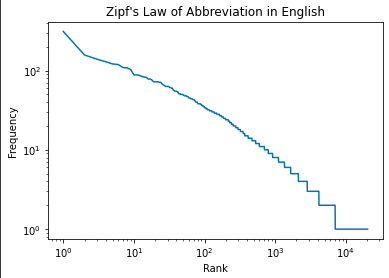
\includegraphics[scale=.60]{ZipfLawInENGLISH}
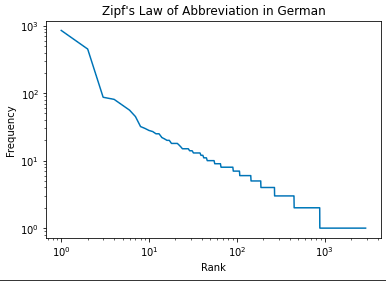
\includegraphics[scale=.60]{ZipfLawInGERMAN}
\end{figure}
\section{Code}

You can find the source code of the project at:\\

\large{{\url{https://github.com/llamas2/zipfsbrevity.git}}

%\section{Conclusion}
%\lipsum[2-8]

%\nocite{bentz2016zipf,Gleason,Hart,Linders,Rich}
\nocite{*}
\bibliographystyle{plain}
\bibliography{referencias}
\end{document}
